\documentclass[a4paper, 12pt]{article}
\usepackage[utf8]{inputenc}
\usepackage[brazil]{babel}
\usepackage{amstext} 	% need for \text command
\usepackage{amsmath}    % need for subequations
\usepackage{graphicx}   % need for figures
\usepackage{verbatim}   % useful for program listings
\usepackage{color}      % use if color is used in text
\usepackage{subfigure}  % use for side-by-side figures
\usepackage{hyperref}   % use for hypertext links, including those to external documents and URLs
\usepackage{pictexwd}	% use for pictex graphs
\usepackage{booktabs}	% use for Publication quality tables in LaTeX

%\author{Vítor M. Martins}
\title{PMR2321}

\begin{document}
\maketitle
%\newpage
%\tableofcontents
%\newpage

\section{Ex 1}

\begin{figure}[h]
\begin{center}
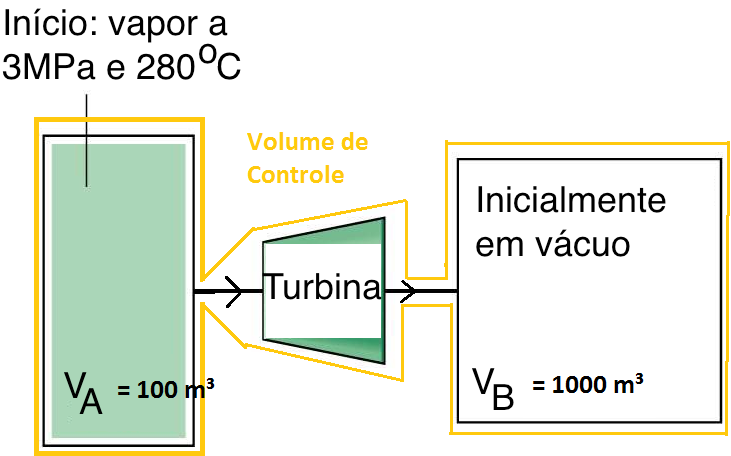
\includegraphics[scale=0.54]{./fig/1.png}
\caption{\label{fig:1} Ex 1} 
\end{center}
\end{figure}

1ª Lei:

\[U_{2}-U_{1}= Q - W \]
Q = 0, logo:
\[W = U_{1}-U_{2}\]

\[W = (U_{A1}+U_{B1})-(U_{A2}+U_{B2})\]
Mas $m_{B1}=0$
\[W = (m_{A1}u_{A1}+m_{B1}u_{B1})-(m_{A2}u_{A2}+m_{B2}u_{B2})\]
\[W=m(u_{1}-u_{2})\]
Devemos minimizar $m_{B1}$ para obter o trabalho máximo

2ª Lei:

\[S_{2}-S_{1}= \int_{}^{} \frac{\delta Q}{\text{T}} + S_{g}\]
\[m(s_{2}-s_{1})=S_{g}\]
\[Tds=du+pdv\]
Onde pdv = 0, já que o volume específico não varia em um volume de controle em que TODO O SISTEMA (Tanque A, Tanque B e Turbina) são meu Volume de Controle, mantendo todo o tempo a mesma massa e o mesmo volume. Portanto Tds cresce com du e $S_{g}=0$,$\ s_{2}=s_{1}$.

Estado 1:

\[v_{1A}= \frac{V_{A}}{m}\]
\[m=\frac{V_{A}}{v_{1A}}\]
\begin{itemize}
\item $u_{1}$=2709.9kJ/kg
\item $v_{1}$=0.0771$m^{3}$/kg
\item $s_{1}$=6.4462kJ/kgK
\end{itemize}
Temos, portanto, vapor superaquecido.

Estado 2:
\[s_{2}=s_{1}=6.4462 kJ/kgK\]
\[v_{2}=\frac{V_{A}+V_{B}}{m}\]
\begin{itemize}
\item $T_{2}$=2709.9kJ/kg
\item $P_{2}$=0.0771 $m^{3}$/kg
\item $x_{2}$=6.4462kJ/kgK
\item $u_{2}$=2270kJ/kg
\end{itemize}
Portanto, W = $5.71 * 10^{5} kJ$

\section{Ex 2} 
\begin{figure}[h]
\begin{center}
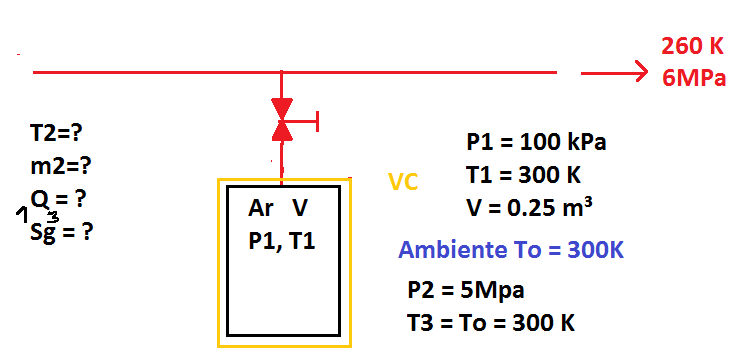
\includegraphics[scale=0.58]{./fig/2.png}
\caption{\label{fig:2}Ex 2} 
\end{center}
\end{figure}

1ª Lei (regime uniforme) (processo $1 \rightarrow 2$ )
\[U_{2}-U_{1}=m_{e}h_{e}\]
\[m_{2}u_{2}-m_{1}u_{1}=(m_{2}-m_{1})h_{e}\]
A 260 k e 6MPa:
\[m_{1}=\frac{P_{1}V_{1}}{RT_{1}}=0.290kg\]
\[u_{1}(T_{1},P_{1})=214.36kJ/kg\]
\[h_{e}(260K)=260.32kJ/kg\]
\[m_{2}=\frac{P_{2}V}{RT_{2}}=\frac{5000*0.25}{0.287*T_{2}}=\frac{4355}{T_{2}}\]

1ª Lei:

\[u_{2}+0.00306 T_{2}=260.32\]

Determinar $u_{2}$ iterativamente através da Tabela \ref{tab:tab1}
% Table generated by Excel2LaTeX from sheet 'Plan1'
\begin{table}[htbp]
  \centering
  \caption{Tabela de Iterações para achar $u_{2}$}
    \begin{tabular}{rrr}
    \toprule
    $T_{2}(k)$ & $u_{2}$ (tabela A7) & 1º Membro \\
    \midrule
    360   & 257,24 & 258 \\
    370   & 264,46 &  \\
    \bottomrule
    \end{tabular}%
  \label{tab:tab1}%
\end{table}%

 \[ T_{2}=362 K\]
Portanto $m_{2}=12.0kg$

\paragraph*{Calculo de $Q_{1 \rightarrow 3}$}

Posso aplicar a 1a lei para o processo $2 \rightarrow 3$ já que o processo $1 \rightarrow 2$ é adiabático (enunciado do exercício)
\[Q_{1 \rightarrow 3} = Q_{2 \rightarrow 3}\]
\[m_{3}u_{3}-m_{2}u_{2}=Q_{2 \rightarrow 3}\]
\begin{itemize}
\item $m_{3}=m_{2}$
\item $u_{3}(T_{3}=T_{0})$
\item $u_{2}(T_{2}=362 K)$
\end{itemize}

\[m_{3}u_{3}-m_{1}u_{1}=(m_{2}-m_{1})h_{e}+Q_{1 \rightarrow 3}\]
Mas:
\[Q_{1 \rightarrow 3} = Q_{2 \rightarrow 3}\]
Portanto: $Q_{1 \rightarrow 3}$=-538kJ

\paragraph*{Calculo de $S_{g}$}

Preciso expandir meu volume de controle desde o reservatório até o lugar geométrico dos pontos de 300 K, de modo a englobar todos os pontos geradores de entropia do meu sistema.
Portanto:

\[m_{3}s_{3}-m_{1}s_{1}=(m_{2}-m_{1})s_{e}+\frac{Q_{1 \rightarrow 3}}{T_{0}}+S_{g}\]
\[m_{3}=m_{2}\]
\[s_{3}(T_{0},P_{3})\]
\[s_{1}(T_{0},P_{1})\]
\[s_{e}(260K,6MPa)\]
\[s_{3}-s_{e}=6.8693-6.7256-R\ln(\frac{4140}{6000})\]
Onde 4140 é $P_{3}$
\[s_{1}-s_{e}=6.8693-6.7256-R\ln(\frac{100}{6000})\]
Resposta: $S_{g}$=4.42 kJ/K


Exercicio para entrega: Repetir esse mesmo exercicio considerando calores especificos constantes



\end{document}